\documentclass[12pt,oneside,letterpaper]{memoir}

\usepackage[T1]{fontenc}
\usepackage[utf8]{inputenc}
\usepackage{microtype}
% \usepackage{kpfonts}

\usepackage{hyperref}
\usepackage{natbib}
\usepackage[table]{xcolor}
% \usepackage{url}
% \usepackage{xurl}
% \usepackage{latexsym,amsmath}
\usepackage{booktabs}
% \usepackage{graphicx}
% \usepackage[nameinlink]{cleveref}
\usepackage{dingbat}
\usepackage{tikz}
\usetikzlibrary{shapes,arrows,shadows,shadows.blur,calc,fit,positioning,mindmap,patterns,scopes,backgrounds}
\usepackage{xurl}            % simple URL typesetting
\usepackage{amsfonts}       % blackboard math symbols
\usepackage{nicefrac}       % compact symbols for 1/2, etc.
\usepackage{fancyvrb}
\usepackage{enumitem}
\usepackage{subcaption}

\usepackage{lipsum}
\usepackage{latexsym,amsmath}
\usepackage{graphicx}
\usepackage{colortbl}
\usepackage{pgfplots}
\usepackage{amssymb}
\usepackage{pgfplotstable}
\usepackage{multirow}

\pgfplotsset{compat=1.18}


\usepackage[capitalise,nameinlink]{cleveref}  % Needs to be last to work.

\usepackage{hyperref}
\usepackage{url}
\usepackage{xurl}
\usepackage{latexsym,amsmath}
\usepackage{booktabs}
\usepackage{graphicx}
\usepackage{subcaption}
\usepackage[nameinlink]{cleveref}
\usepackage{enumitem}
\usepackage{xcolor}
\usepackage{colortbl}
\usepackage{pgfplots}
\usepackage{amsmath,amssymb}
\usepackage{pgfplotstable}
\usetikzlibrary{shapes,arrows,shadows.blur,calc,positioning,fit}

\pgfplotsset{compat=1.18}

\usepackage{enumitem}
\usepackage{multirow}

\DeclareMathOperator*\mean{\text{mean}}
\DeclareMathOperator*\stdev{\text{stdev}}

\pgfplotsset{
  discard if not/.style 2 args={
    x filter/.code={
      \edef\tempa{\thisrow{#1}}
      \edef\tempb{#2}
      \ifx\tempa\tempb
      \else
        \def\pgfmathresult{inf}
      \fi
    }
  }
}


%%% End Commands %%%

% From Siavoosh Payandeh Azad: https://www.siavoosh.com/blog/2019/01/05/latex-table-cell-coloring-based-on-values-in-the-cell/

% \colorlet{BestColor}{blue!40}
% \colorlet{WorstColor}{red!40}
\definecolor{BestColor}{rgb}{0.5, 0.7, 1.0}
\definecolor{WorstColor}{rgb}{1.0, 0.7, 0.5}

\newcommand{\gradientcell}[3]{
    % The values are calculated linearly between \minval and \maxval
    % \pgfmathparse{int(round(100*(#1/(#3-#2))-(\minval*(100/(#3-#2)))))}
    \pgfmathparse{int(round(100*(#3-#1)/(#2-#1)))))}
      \xdef\tempa{\pgfmathresult}
      % \cellcolor{blue!40!white!\tempa!red!40}
      \cellcolor{BestColor!\tempa!WorstColor}
      % \cellcolor{#5!\tempa!#4!#6} #1
 }

\tikzset{/num grad/.style n args={3}{
  column name=#1,
  column type=r, fixed, fixed zerofill, precision=2,
  postproc cell content/.append style={
    /pgfplots/table/@cell content/.add={\gradientcell{#2}{#3}{##1}}{},
  },
}}



%%% Formatting %%%

\usepackage{inconsolata}
% \usepackage{libertine} % Font
% \usepackage[bitstream-charter]{mathdesign}
% \usepackage{XCharter} % Needed to fix issues with mathdesign
% \usepackage{fourier-otf}
% \usepackage{charter}
% Going with Computer Modern so I stop getting distracted by fonts.

% Margins
\setlrmarginsandblock{1in}{*}{*}
\setulmarginsandblock{1in}{*}{1}

% Headers/Footers
\newcommand\draftdate{\color{gray}\today{} (draft)}
\makeoddfoot{ruled}{\draftdate}{}{\thepage}
\makeatletter
\makepsmarks{ruled}{%
  \nouppercaseheads
  \createmark{chapter}{left}{shownumber}{\@chapapp{} }{. \space}
}
\makeatother
\makeoddhead{ruled}{}{}{\leftmark}
\makeoddfoot{plain}{\draftdate}{\thepage}{}
\pagestyle{ruled}

\checkandfixthelayout

%%% End Formatting %%%


\newif\ifshowcomment

\newcounter{comment}
\newcommand\bjb[1]{{\stepcounter{comment}\color{purple}[BJB\@: #1]}}
\newcommand\drm[1]{{\stepcounter{comment}\color{orange}[DRM\@: #1]}}
\newcommand\cmt[1]{{\stepcounter{comment}\ifshowcomment\color{gray}[:#1]\fi}}

\newcommand\note[1]{\color{gray}[#1]}

\newcommand\inputsrc[1]{\input{#1}}

%%% Matplotlib block %%%
\def\mathdefault#1{#1}
\everymath=\expandafter{\the\everymath\displaystyle}

\ifdefined\pdftexversion\else  % non-pdftex case.
  \usepackage{fontspec}
\fi
\makeatletter\@ifpackageloaded{underscore}{}{\usepackage[strings]{underscore}}\makeatother
%%% end block %%%


\let\abstractOrig\abstract
\let\endabstractOrig\endabstract
\renewenvironment{abstract}{\abstractOrig\noindent\ignorespaces}{\endabstractOrig}


\begin{document}


\thispagestyle{title}
\begin{centering}
\textbf{\LARGE Principled Evaluation of Deep Learning-Based Emergent Communication}

\vspace{3pc}
{\large Brendon J. Boldt}

\vspace{2pc}
\today{}

\vfill

Language Technologies Institute \\
Carnegie Mellon University \\
Pittsburgh, Pennsylvania

\vspace{4pc}

\textbf{Thesis Committee}
\vspace{0.5pc}

\begin{tabular}{lr}
  David Mortensen, \emph{Chair} & Carnegie Mellon University \\
  Yonatan Bisk & Carnegie Mellon University \\
  Katia Sycara & Carnegie Mellon University \\
  Kenny Smith & University of Edinburgh
\end{tabular}

\end{centering}



\newpage
\thispagestyle{plain}
\section*{Abstract}
Emergent communication is the field of research which studies how language-like communication systems evolve from scratch in agent-based simulations.
The most recent incarnation of this topic, starting in 2016, has focused on leveraging recent advancements in deep neural network, reinforcement learning, and natural language processing.
Emergent communication, as a method, has significant potential applications from powering unprecedentedly detailed simulations of how human invent, acquire, and use language to providing an alternative source of language data to the Internet-gulping large language models.
Despite this potential, the field has yet make any significant progress towards these applications largely because it lacks any methodological resources to unify research efforts within the field;
  that is, research findings are often ``one-off'', lacking any way of making general claims or comparing itself directly to other approaches.
This thesis advances the field of emergent communication by developing the resources that are necessary for forging a unified research program that is critical the advancement of any field of science or engineering.

The first contribution is to the conceptual foundations of emergent communication in the form of a comprehensive account of potential applications of emergent communication across natural language processing, multi-agent reinforcement learning, linguistics, and beyond.
\cmt{Include explicit summary of TMLR paper in introduction somewhere?}
This conceptual foundation is paired with the more mundane but entirely vital data resource of a collection of emergent communication corpora collected from a variety of free and open source implementations of simulations from the literature.
These two elements in turn enable the introduction of \emph{evaluation} metrics---that is, quantitative measures of emergent communication which quantify how good, in some general sense, a language generated by an emergent communication simulation is.
In particular, we quantify ``how good an emergent language is'' by measuring its similarity to human language.
This is done in two complementary paradigms: a data-driven, machine learning paradigm and a theoretically-motivated linguistic paradigm.
The machine learning-based metric uses deep transfer learning to assess how similar an emergent language is to human language by using the emergent language as pretraining data for a downstream human language-based task.
The linguistics-based metrics algorithmically identify the presence of universal features of human language in emergent languages.
Finally, this thesis explores the relationship between the machine learning-based and linguistics-based metrics, so as to determine what types of emergent communication simulations produce the most human language-like emergent languages in a general sense.


\newpage
\tableofcontents*

\setcounter{chapter}{-1}
%%%%%%%%%%%%%%%%%%%%%%%%%%
\chapter{Proposal Summary}
%%%%%%%%%%%%%%%%%%%%%%%%%%

This chapter will not be part of the final thesis but serves as more of an executive summary of where I am in the thesis process.
\Cref{tab:timeline} describe the notional timeline of my doctoral work.
The following to sections briefly summarize the papers I have completed so far, and the papers that I plan to publish to complete my thesis.
More substantial descriptions of the work are given in the body of thesis.


\begin{table}
  \centering
  \begin{tabular}{lll}
  \toprule
  2019  & August            & Began research master's degree (CMU) \\
  2021  & August            & Completed masters, began PhD \\
  % 2024  & July--September   & XferBench eval (\Cref{ch:hpo}) \\
  2025  & January           & Proposal \\
        & January--March    & Rich corpora (\Cref{ch:rich-corpora}) \\
        & April--June       & Morphemes (\Cref{ch:morphemes}) \\
        & July--September   & Morpheme structure (\Cref{ch:syntax}) \\
        & September         & Defense \\
  \bottomrule
  \end{tabular}

  \caption{Timeline of proposed work and thesis completion.}
  \unskip\label{tab:timeline}
\end{table}

\section{Completed Work}
% The following completed research papers will be incorporated into the thesis (either in part or their entirety).
% Other work has be published and/or completed during the course of my master's and doctoral work but will not play major role in the thesis.


\subsection{Recommendations for Systematic Research on Emergent Language}
\noindent
\citet{boldt2022recommendations} was rejected from ICML 2022; part of this work was expanded into ``A Review of the Applications of Deep Learning-Based Emergent Communication'' discussed below.
This is a position paper which critiques and makes recommendations for emergent communication research from a meta-scientific angle.
It begins by specifying the goals of emergent communication research (which would eventually become the TMLR paper).
In light of these goals, which are split between ``engineering'' and ``scientific'' goals, the paper discusses core methodological elements of engineering and science.
Finally, each of the core methodological elements is explicitly detailed in the context of emergent communication.
In addition to the goals, the particular elements of engineering which are pursued in this thesis are evaluation metrics and standard datasets.

\subsection{A Review of the Applications of Deep Learning-Based Emergent Communication}

\noindent
\citet{boldt2024review} was published in the \textit{Transactions of Machine Learning Research} (TMLR) in February 2024.
This paper comprehensively reviews the applications and goal of emergent communication research drawing on both the literature and the author's (i.e., Brendon and David's) experience in the field.
Each application, in addition to a description and review of the relevant literature, is a accompanied by a brief set of recommendations on the most fruitful next steps for that research direction.
The set of applications themselves is divided into three categories:
  (1) internal applications, which focus on improving the methods of emergent communication itself,
  (2) task-driven applications, which look at engineering tasks focused on more effectively solving particular problems,
  and (3) knowledge-driven applications, which aim at increasing scientific understanding of particular phenomena.

\subsection{XferBench: a Data-Driven Benchmark for Emergent Language}
\noindent
\citet{boldt2024xferbench} was published in the \textit{Proceedings of the 2024 Conference of the North American Chapter of the Association for Computational Linguistics: Human Language Technologies (Volume 1: Long Papers)} (NAACL).
This paper introduces a first-of-its-kind evaluation metric/benchmark for emergent languages.
It addresses the question of the \emph{quality} of an emergent language by looking at its similarity to human language from a data-driven, machine learning perspective.
Specifically, it quantifies ``similarity to human language''---and, therefore, overall quality---as how much pretraining on an emergent language corpus improves performance on modeling human language (although we also test machine translation).
XferBench is published as an easy-to-use Python package, and since it only requires an unannotated corpus of utterances from the emergent language, it is intended to have widespread use in emergent communication research.


\subsection{ELCC: the Emergent Language Corpus Collection}
Under review at the \textit{2025 International Conference on Learning Representations} (ICLR; decision in January 2025).
This paper introduces a collection of over $70$ emergent language corpora from across $8$ different systems in the literature.
Each of these corpora is annotated with statistical analyses as well as metadata documenting the features of the system/environment it came from.
Such a resource is intended to make studying emergent languages themselves far easier since it obviates the need run the systems oneself and enables comparative studies given the variety of emergent communication systems included.

\subsection{Searching for the Most Human-like Emergent Language}
Under review in the December 2024 cycle of the \emph{Association for Computational Linguistics (ACL) Rolling Review}.
This paper uses Bayesian hyperparameter search on a signalling game-based emergent communication environment to generate languages which perform well on XferBench (i.e., transfer well to human language modelling).
The experiments result in state-of-the-art emergent languages for transfer learning even surpassing one of the anomalously low human language baselines.
This process also yields concrete recommendations on what hyperparameter settings lead to emergent languages more statistically similar to human languages.
Finally, this experiments reveal that there is a significant correlation between emergent language entropy and its performance on XferBench, suggesting that entropy is ``minimized'' with respect to transfer learning performance.

\subsection{Other Work}
Some work completed during the course of master's and doctoral work will not factor heavily into the thesis.
In ``Mathematically modelling the lexicon entropy of emergent language'' \citep{boldt2022mathematically}, we investigate using a formal model based on the Chinese restaurant process to make predictions of the entropy of lexica in emergent languages; this is intended to be a sort of exemplar of using formal models to make clear, determinate hypotheses regarding emergent communication experiments.
In ``Shaped rewards bias emergent language'' \citep{boldt2022shaped}, we argue that reward shaping (a common feature of reinforcement learning experiments) has the potential to bias (i.e., predetermine) properties of the resulting emergent language.
In ``Case study: deontological ethics in NLP'' \citep{prabhumoye-etal-2021-case}, we apply deontological approach to ethics to different real-world scenarios in natural language processing-based systems.



\section{Proposed Work}
This section will briefly described the proposed work for the completion of the doctoral thesis.
Each of these papers is intended to a standard conference-length paper (i.e., 8--9 pages).


\subsection{Rich emergent language corpora}
ELCC, the current collection of emergent language corpora, only includes the corpora themselves and aggregate statistics, but many interesting research directions require not only having access to the tokens of utterances themselves but also their context.
For example, anything related to semantics is going to require some way to determine what an utterance means.
Thus, we propose an extension to ELCC which takes the same set of corpora and includes information about the state of the environment before and after each utterance so as to supply grounding for each of the utterances.
From here, it will be possible to explore a far greater range of phenomena with respect to the emergent language corpora in ELCC\@.

\subsection{Automatically detecting morphemes in emergent language corpora}
While the original plan was to create a linguistic counterpart to XferBench, that is, some benchmark-like metric which measured the presence of human language-like linguistic structures in emergent communication, I rolled back my ambition considerably as there are not yet methods for detecting structure in emergent communication generally.
Thus, this project will make an important step in the direction of such a metric by introducing and testing an algorithm to detect and segment emergent communication utterances into morphemes: particular meanings paired with an atomic form.
Understanding (and identifying) morphemes in emergent language is critical to understanding many (if not the majority of) linguistic phenomena from morphology to syntax to discourse; double articulation a fundamental feature of human language.
Yet there are no existing methods determining what the meaningful units of an emergent communication utterance are in a general, system-agnostic way (e.g., is each token its own morpheme are they sub-morpheme units?).
This work will leverage the rich emergent language corpora discussed above as it is necessary to pair the utterances (form) with the accompanying context (meaning) in order to uncover morphemes (or at least an analogous structure).
Being able to turn emergent languages represented as strings of raw tokens into strings of morphemes will enable more principled research on linguistic structures which presuppose the existence and identification of morphemes (e.g., syntax).


\subsection{Automatically detecting morpheme structure}
Building on the above chapter detecting morphemes, this chapter will use a somewhat similar approach to detect structural features in emergent language corpora.
Namely, the strings of morphemes from the previous method are first mapped to classes (determined, mostly, by the semantics of the morphemes) which are then run through decision functions which detect structural features (e.g., one morpheme class succeeding another).
These structural features are then generalized into patterns using a statistical measure (e.g., mutual information).
The algorithm, then, yields a list of significant morpheme patterns found in the emergent language corpus.
This chapter stops short of claiming that what is being detected is ``syntax'' in any linguistically robust sense and instead focuses on a more minimalist notion of structure.
Down the road, and beyond the scope of this thesis, this method could be incorporated into a broader account of syntax.



%%%%%%%%%%%%%%%%%%%%%%
\chapter{Introduction}
%%%%%%%%%%%%%%%%%%%%%%

Modern-day large language model-based AI systems are good a mimicking human language.
Some might even say they are good at \emph{using} human language, but this is either imprecise or inaccurate:
  LLMs' production of text is based the statistical likelihood of meaningless (so far as they are concerned) tokens, fine-tuned to humans' preferences.
This is in contrast to humans' use---and event more so their acquisition---of language which is laden with meaning derived from the rich internal, physical, and social context which permeates language use.
The end result is that LLMs' approximation of human language fails at a number of tasks, but, more significantly, falls short in providing insights into the nature of human language itself.

\emph{Emergent communication} (also known as \emph{emergent language}) is an alternative paradigm to developing language-capable models that does not does not train on human language data but rather invents a communication system \emph{de novo}.
In its most basic form, emergent communication comprises a simulation using neural network-based agents which are trained to cooperatively complete some task in a virtual environment.
These agents are equipped with a communication channel of discrete tokens with no \emph{a priori} meaning---the meaning of communication is established through the optimization process encouraging communication which is advantageous to completing the task.
% The communication protocol, then, is the ``emergent language'' since the meaningful system of communication as arisen organically from the environment and task.

Emergent communication differs from the more ``traditional'' approach to language that LLMs use in that it does not try mimic human language but instead tries to rederive language from similar function pressures which are hypothesized to have guided human language's own evolution.
Since the process language emerging is far more analogous to how human language develops and is learned, it has a much greater potential to yield significant gains the scientific understanding of human language.
Furthermore, certain practical tasks might lie beyond the reach of the mimicry approach LLMs employ due to surface-level operations; these problems, too, can be addressed by emergent communication which models not only the surface features of language but also its semantics and social context.
Finally, generating language data through emergent communication avoids many of the ethical issues that crop up with LLMs dependence on human language data from amplifying toxicity from the Web to freely (ab)using copyrighted and personal content \citep{weidinger2021ethicalsocialrisksharm,carlini2021extractingtrainingdatalarge}.

Here is the problem: the field of emergent communication has not yet solved any problems either in the area of scientific understanding nor in practical applications.
Furthermore, it has not even shown measurable progress towards these goals either.
This thesis, then, establishes methods in emergent communication that enable measurable progress in emergent language research so as to move the field towards solving practical applications and improving scientific understanding.
It does this by first introducing emergent language data resources which permit empirical evaluation across a variety of emergent languages.
These resources are then used to develop
  (1) a deep transfer learning-based evaluation metric for emergent communication to measure the practical applicability of emergent language
  and (2) algorithms for characterizing the morphology of emergent languages as a foundation for further linguistic analysis.

\section{Background}

The field of deep learning-based emergent communication has its genesis in 2016 with papers including
  ``Learning to communicate with deep multi-agent reinforcement learning'' \citep{foerster2016learning}
  and ``Multi-Agent Cooperation and the Emergence of (Natural) Language'' \citep{lazaridou2016multiagent}.
These were the first paper to combine combine deep learning, and specifically deep reinforcement learning, to developing discrete token-based communication systems from scratch.
While prior work applied mathematical models \citep{brighton2005} and classical machine learning methods \citep{werner_Dyer_1991}, the introduction of deep learning opened up the possibility of a far more robust notion of the results of the simulations being \emph{emergent}.
That is, with mathematical models the range of results is tightly constrained by the design of the model and ``emergent'' phenomena are either relatively simple or encoded into the model itself.\footnote{Although Conway's Game of Life is notable exception to this.}
Deep reinforcement learning, on the other hand, has demonstrated vivid example of complex behaviors emerging in environments with simple rules such as DeepMind's AlphaZero \citep{silver2017masteringchessshogiselfplay} or OpenAI's multi-agent hide-and-seek \citep{baker2020emergenttoolusemultiagent}.

The prototypical emergent communication experiment consists two or more deep neural network-based agents situated in some kind of environment or game where they must cooperate in order to succeed.
The agents are equipped with a communication channel consisting of discrete tokens with no \emph{a priori} meaning; it is only through the reinforcement learning-based optimization that messages passed between agents begin to take on meaning.
The resulting behavior, most especially the communication protocol, is the typically the object analysis, addressing question such as:
  Did an effective communication protocol emerge at all?
  What structural features characterize it?
  Do these features align at all to human language?
  What can we infer about language formation more generally from the above?

In practice, much of the literature has focused on the signalling game and the emergence of compositionality in communication (jointly and separately)
  \citep{havrylov2017sequence,mordatch2018grounded,chaabouni2022emergent}.
The signalling game was introduced in the context of game theory by David Lewis \citep{lewis1970ConventionAP}.
The signalling game is one of the simplest possible environments for emergent communication contributing, in large part, to its popularity.
It consists of only two agents: a sender and a receiver.
The sender makes on observation (e.g., an orange circle) and sends a message to the receiver who must, based on the message alone, determine the nature of the observation (e.g., it was an orange circle, not a blue circle).
A visualization of the signalling game is provided in \Cref{fig:signaling-game}.
The question of compositionality arises when we look at how the communication protocol encodes compound meanings like a red square: A compositional protocol would encode ``red'' and ``circle'' with their own words which could be reused to express meanings like a red circle or a blue square.
On the other hand, holistic communication sometimes emerges where a unique word refers to red square, bearing no relation to the word(s) for red circle.
Compositional communication, generally, is seen as more desirable both for practical reasons (more efficient encoding of information) as well as for its resemblance to how humans tend to encode meaning in language.

\begin{figure}
  \centering
  \begin{subfigure}[b]{0.53\textwidth}
    \centering
    \setlength\fboxsep{0pt}
    \def\cubeoffset{0.25}
\tikzset{
  boxface/.pic={
    \fill
      (0,0)
        edge (1,0)
        edge (0,1)
        edge (0-\cubeoffset,0+\cubeoffset)
      (1,1)
        edge (1,0)
        edge (0,1)
        edge (1-\cubeoffset,1+\cubeoffset)
      (0-\cubeoffset,1+\cubeoffset)
        edge (0-\cubeoffset,0+\cubeoffset)
        edge (1-\cubeoffset,1+\cubeoffset)
        edge (0,1)
      ;

    \fill (0.3, 0.7) circle [radius=0.03];
    \fill (0.7, 0.7) circle [radius=0.03];

    \path [] (0.3, 0.3) edge (0.7, 0.3);
  }
}

\begin{tikzpicture}[scale=0.8, transform shape]

  \node (t1) at (-4, 0.5) {\large$T_1$};
  \draw (-\cubeoffset,0) pic [xscale=-1] {boxface};
  \fill [orange!60] (-3, 0.5) circle [radius=0.4];
  \node at (-1.9, 0.5) {\Large\eye};
  \draw (3,0) pic {boxface};
  \draw [gray] (-3.5, -0.4) to (4.8, -0.4);

  { [yshift=-2cm]
    \node (t2) at (-4, 0.5) {\large$T_2$};
    \draw (-1,0) pic {boxface};
    \node[rectangle callout, draw, callout absolute pointer={(0.1,0.5)}] at (1.3,1) {3 14 1 59 2};
    \draw (4-\cubeoffset,0) pic [xscale=-1] {boxface};
    \draw [gray] (-3.5, -0.4) to (4.8, -0.4);
  }

  { [yshift=-4cm]
    \node (t3) at (-4, 0.5) {\large$T_3$};
    \draw (-1,0) pic {boxface};
    \draw (3,0) pic {boxface};
    \node (opt1) [fill=orange!60,regular polygon, regular polygon sides=4, inner sep=0.25cm] at (5.5, 1.5) {};
    \node (opt2) [fill=blue!60,below=0.5cm of opt1,circle,inner sep=0.25cm,anchor=center] {};
    \node (opt3) [fill=orange!60,below=0.5cm of opt2,circle,inner sep=0.25cm,anchor=center] {};
    \node [left=0.0cm of opt3,anchor=east,yshift=-1.5mm] {\Large\leftpointright};
  }

  \draw [-stealth, black!50, dashed] (t1) to (t2);
  \draw [-stealth, black!50, dashed] (t2) to (t3);

\end{tikzpicture}

    \vspace{1cm}
    \caption{%
      $T_1$: The sender (left) observes an object.
      $T_2$: The sender passes a message to the receiver (right).
      $T_3$: The receiver chooses from a handful of candidate objects.
    }
    \unskip\label{fig:boxface}
  \end{subfigure}
  \hfill
  \begin{subfigure}[b]{0.45\textwidth}
    \centering
    \tikzstyle{blockStyle}=[
  draw=black!50,
  text width=2.7cm,
  minimum width=2cm,
  text centered,
  rounded corners,
  font=\scriptsize,
]

\newcommand\blocktext[2]{\textsc{#1}\\{\color{black!70}#2}}

\begin{tikzpicture}
  [node distance=3mm, outer sep=0mm, inner xsep=-1mm]

  \node (obs) [blockStyle] {\blocktext{Observation}{vector}};
  \node (sender) [blockStyle,below=of obs.south] {\blocktext{Sender}{RNN conditioned on observation}};
  \node (message) [blockStyle,below=of sender.south] {\blocktext{Message}{sequence of one-hot vectors}};
  \node (distobs) [blockStyle,right=of message.east] {\blocktext{Candidate\\Observations}{set of vectors}};
  \node (n0) at ({$(message)!.5!(distobs)$} |- {message.south}) {};
  \node (receiver) [blockStyle,below=of n0] {\blocktext{Receiver}{RNN conditioned on message and observations}};
  \node (pred) [blockStyle,below=of receiver.south] {\blocktext{Prediction}{prob.\@ dist.\@ over observations}};
  \node (reward) [blockStyle,below=of pred.south] {\blocktext{Reward}{real value}};

  \draw [-stealth] (obs) to (sender);
  \draw [-stealth] (sender) to (message);
  \draw [-stealth] (message) to (receiver);
  \draw [-stealth] (distobs) to (receiver);
  \draw [-stealth] (receiver) to (pred);
  \draw [-stealth] (pred) to (reward);
  \draw [-stealth, bend left, dashed] (obs.east) to (distobs);
  \draw [-stealth, dashed, inner sep=0mm] (reward.west) to[looseness=0.8, out=135, in=225] (sender.south west);
  \draw [-stealth, dashed] (reward.west) to[looseness=1, out=135, in=225] (receiver.west);

  \clip (obs.west |- obs.north) rectangle (distobs.east |- reward.south);
\end{tikzpicture}

    \caption{Illustration of the technical architecture of the signaling game.}
    \unskip\label{fig:signaling-chart}
  \end{subfigure}
  \caption{%
    An illustration of the discrimination variant of the signaling game, one of the simplest and most common environments in emergent communication research.
  }
  \unskip\label{fig:signaling-game}
\end{figure}


Other environments do appear in the literature such as navigation tasks or dialogue-based games
  \citep{unger2020GeneralizingEC,brandizzi2022rlupus}.
In addition to compositionality, other phenomena have been the subject of investigation such as pragmatics, transfer learning, and the information theoretic properties of emergent language
  \citep{kang2020incorporatingpragmaticreasoningcommunication,yao2022linking,tucker2021discrete}.
While there are too many papers to summarize comprehensively here, I estimate that there are on the order of $200$ papers directly related to emergent communication.\footnote{Figure based on finding ${\sim}150$ papers during a comprehensive literature review in 2023.}
For a general review of the emergent communication literature, I recommend \citet{lazaridou2020emergentmultiagentcommunicationdeep}.

\section{Motivation}

In the seven or so years of deep learning-based emergent communication's existence, there has been little concrete progress in the field.
Much of the research has focused on addressing small-scale, isolated phenomena without a way to unify the findings into a broader understanding.
While normal science (as Kuhn terms it \citep{kuhn}) often proceeds by small, additive research contributions, emergent communication has not developed paradigm where the small contributions can truly add together.
One can read much of the literature on emergent communication, learn of many different trends that appeared in particular environments, and still largely have no idea why emergent languages look the way they do nor what they might look like in a new environment.
Furthermore, despite the potential for groundbreaking applications in natural language processing and linguistics, emergent communication has not yielded any substantial contributions either \citep{boldt2024review}.

This thesis is intended to make foundational contributions addressing the unique structural issues in emergent communication research that has resulted in this.
If the same old, tried and true methods of machine learning simply worked for emergent language, we would have seen tangible progress by now, but we have not, so one can assume that emergent language is a dead end, is missing a key technological prerequisite (e.g., computing resources, better reinforcement learning algorithms), or needs specially tailored methodological improvements.
This thesis is an attempt at the last of these.
In particular, the overall intent of the thesis is to create quantitative evaluative methods which work across a wide variety of emergent communication environments in order to support a research and development workflow more like that of the rest of deep learning-based research.
Methods should yield \emph{quantitative} metrics to permit direct comparison of different systems, statistical analysis, and more automated methods of exploring emergent communication environments.
These methods must also be \emph{evaluative} since we a number that we can optimize for---a goal---not simply a number describing one aspect of a system that requires further interpretation.
Finally, this thesis looks to rest of deep learning research, especially in regards to structures like benchmarks and evaluation metrics, for inspiration because these factors are critical for its own success.
While the long-term development of emergent communication methods needs far more than just borrowing methods from deep learning, developing general-purpose evaluative tools is critical in unifying the research efforts of the field such that they can begin to progress in a tangible way.

\paragraph{An aside}
While the fundamental lack of progress has, from an early point, been the main focus of my doctoral research, I had to make a decision between two ways of addressing this problem: the ``scientific'' way and the ``engineering'' way.
The scientific approach would entail developing a theory of emergent communication which would enable progress by first creating a concrete, unified theory that research could contribute two, and second, by illuminating the most promising directions based on the predictions of the field.
Such an approach was addressed by my paper ``Mathematically Modeling the Lexicon Entropy of Emergent Language'' \citep{boldt2022mathematically} which was a sort of proof-of-concept for this approach, attempting to establish an empirically verifiable formal model of certain behaviors in emergent communication experiments.
Of the two approaches, this one certainly had (and has) more appeal to me, but I ultimately decided against it largely because I judged that it was not feasible.
In essence, the current paradigm of emergent communication research follows this approach (even if the scientific method is hardly employed explicitly), that is, trying to find general principles which can be empirically verified.
I think this paradigm fails in large part because emergent language is\dots\emph{emergent}!
No amount of adding up little parts is going to tell you ahead of time what is going to happen in the large-scale, so the idea would go.
If this is true, and my intuition pushes me in this direction, then emergent communication, \emph{qua} emergent phenomenon, is a matter of ``go big or go home'': scale up or pack up.\footnote{This sounds like a bitter lesson \citep{bitter-lesson}.}

This leads us to the engineering approach which might be summed up as: how to scale up intelligently.
This is the approach this thesis follows.
In contrast to the scientific approach, the engineering approach focuses on creating structures which allow research to try a wide variety of approaches and efficiently sift through the results to find the next handhold in the ascent.
Naturally, some degree of theoretical understanding is necessary to explore intelligently, but the threshold of understanding for guiding exploration is lower than what might typically be associated with scientific understanding or prediction.
Finally, from a practical standpoint, the engineering approach proved more tractable for writing a thesis: the intermediate papers more easily speak for themselves and making an immediate impact is far more feasible.



\section{Overview}

This thesis has three main parts:
The first comprises \Cref{ch:elcc,ch:rich-corpora}, which introduce a large collection of emergent language corpora and corresponding semantic annotations.
Second, \Cref{ch:xferbench,ch:hpo} introduce and showcase XferBench, a deep transfer learning-based evaluation metric for emergent language corpora.
Lastly, \Cref{ch:morphemes,ch:syntax} introduce methods for detecting linguistic structures in emergent language corpora.
Each of these parts largely stands on its own for the purposes of readability as well as their contributions.
Nevertheless, the entire thesis is intended to provide a coherent, multi-pronged approach to the problem of a lack of measurability of progress.


\subsection{Data resources for emergent language}
\Cref{ch:elcc,ch:rich-corpora} introduce an important data resource to emergent communication research: the Emergent Language Corpus Collection (ELCC), a collection of emergent language corpora with semantic annotations of utterances derived from a variety of free and open source emergent communication implementations.
Each of these corpora is accompanied by metadata describing statistical properties of the corpus, taxonomic properties of the environment it came from, and a turnkey shell script for reproducing the corpus (or developing a new one).
This collection of corpora is made a public such that it can be both easily used and contributed to by the broader research community.

In its own right, this collection is a significant contribution to emergent communication as it increases the accessibility of emergent language data both for researchers who might be able to generate the emergent languages themselves and those looking to compare a wide variety of emergent languages.
More importantly for the thesis, though, having a robust collection of emergent language corpora is necessary test, contextualize, and motivate the results of the following chapters.
The transfer learning-based metric discussed below takes emergent language corpora as input, and to demonstrate its utility in comparing various approaches to emergent communication, it needs to be applied to a wide variety of emergent languages.
For the methods of detecting linguistic structure, not only is the variety of emergent languages important, but the semantic annotations are a critical part of discovering the latent structure that might be present in the emergent languages.
Thus, the collection of emergent language corpora forms the foundation for the rest of the research in this thesis while also demonstrating how emergent communication research can be made more accessible.

\subsection{Transfer learning-based evaluation}

\Cref{ch:xferbench,ch:hpo} introduce XferBench, an evaluation metric for emergent language corpora based on deep transfer learning.
The intuition behind XferBench is that when a model is pretrained on emergent language data, its downstream performance on human language-based natural language processing tasks (e.g., language modelling, machine translation) is correlated with its similarity to human language, as far as a deep neural network is concerned.
XferBench is packaged as a benchmark: standardized data and settings with a clean, easy-to-use implementation to permit widespread.

XferBench exemplifies the goal of the thesis insofar as it establishes an evaluative method for easily and effectively comparing emergent languages on a level playing field.
The transfer learning-based approach captures notion of how ``good'' an emergent language (corpus) is from the perspective of machine learning.
This is meant in two ways:
  First, the emergent languages are analyzed according to the methods of machine learning, discovering regularly occurring patterns with data-driven methods and a low inductive bias.
  Second, transfer learning method closely mirrors many of the practical applications of emergent communication which consist of using emergent language data is pretraining or evaluation data for natural language processing models.
While it is not as simple to establish a ranking of ``better'' and ``worse'' with the largely open ended task of designing an emergent communication environment, XferBench still provides a useful notion of what directions are having a tangible effect on the complexity of the emergent languages those environments develop.


\subsection{Detecting linguistic structures}

\Cref{ch:morphemes,ch:syntax} introduce algorithms for detecting linguistic structures in any emergent language corpora that possesses in annotations as described above in ELCC.\@
\Cref{ch:morphemes} specifically looks at detecting ``morphemes'' in the sense of atomic units of form with a distinct meaning.
The output is a list of token sequences which correspond with particular meanings in the environment.
Not only does this enable a host of interesting analyses, but it also lays the groundwork for \Cref{ch:syntax} which introduces an algorithm to detect structure among these morphemes, making a first step towards identifying the syntax of emergent languages.

The original intent for the linguistics-focused component of this thesis was to develop a benchmark similar in intent to XferBench but looking at how close the linguistic features of emergent language were to those of human language in areas such as syntax, social variation, and discourse.
Yet upon planning the concrete details of such a metric, it was apparent that it was not clear \emph{if} such features as syntax or discourse existed in any meaningful way, let alone there being a way to detect them.
Thus, in order to help decide where to begin we visualized and informal hierarchy of linguistic phenomena in \Cref{fig:linguistic-dag}; the direction of the hierarchy is determined by what phenomena presuppose the existence of more basic phenomena.
What was immediately apparent is that while it easy to point to concrete notions of semantics and tokens (the atomic components of a message/utterance in emergent communication), even even the existence and nature of the immediate combination of these---morphemes---was not established (and hardly explored).

\begin{figure}
  \centering
  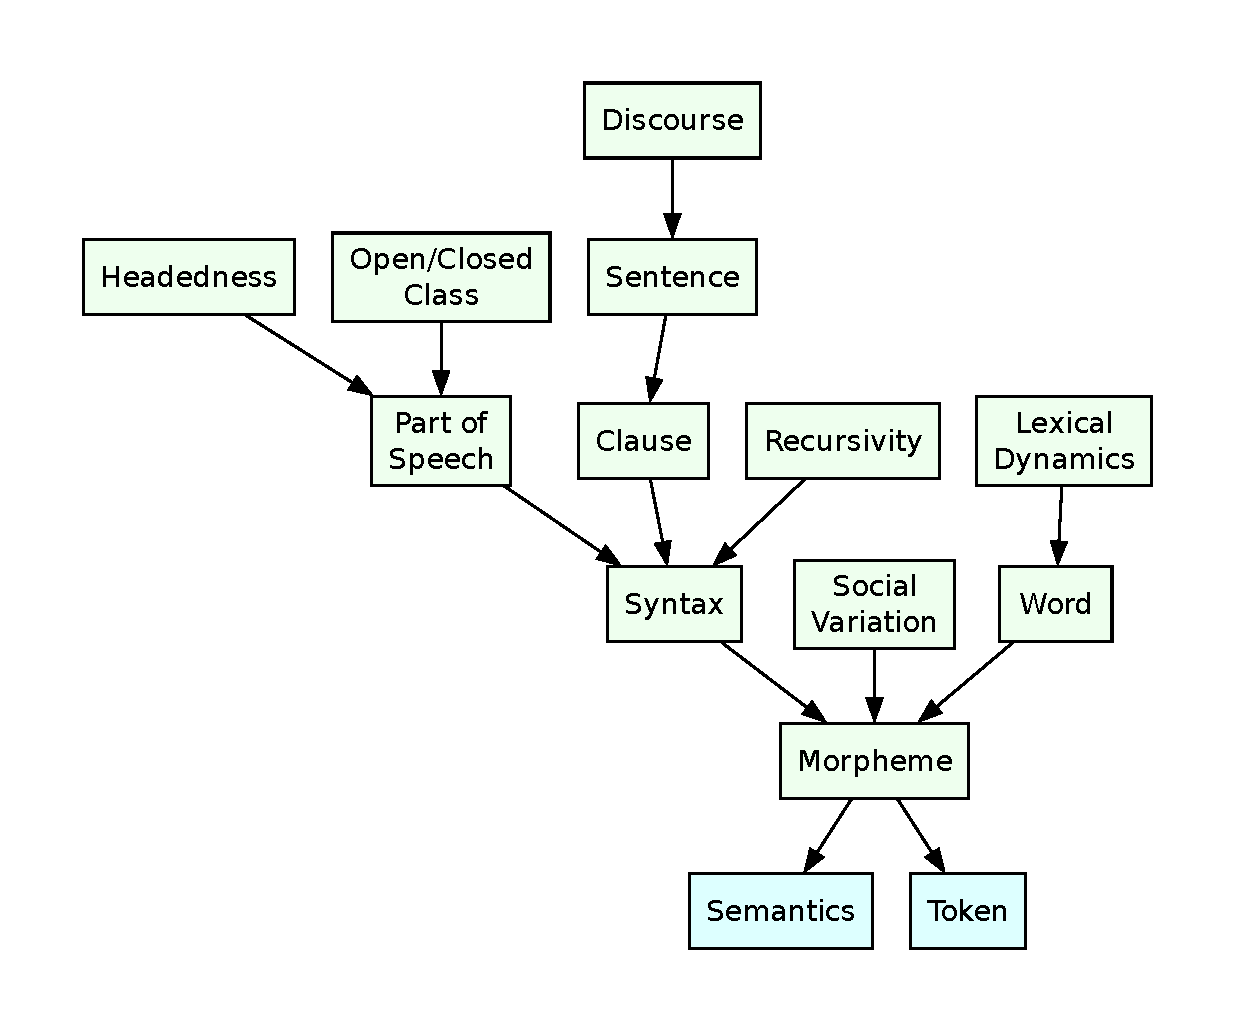
\includegraphics[width=0.85\linewidth]{assets/linguistic-dag}
  \caption{%
    Hierarchy of linguistic concepts.
    $X\rightarrow Y$ can be read as ``the definition of $X$ presupposes $Y$ being defined'' or roughly ``$X$ depends on $Y$''.
    The only concepts whose existence is established in emergent language are \emph{semantics} and \emph{token}.}
  \unskip\label{fig:linguistic-dag}
\end{figure}

Thus, I decided to pursue establishing a method to show the existence of and identify morphemes and syntax---the backbone of the hierarchy depicted in \Cref{fig:linguistic-dag}, which is likely the most that can be done toward developing a metric of linguistic similarity in the scope of this thesis.
Nevertheless, the proposed algorithms still fit well within this thesis' theme of pioneering accessible general purpose in methods in emergent communication that permit the direct comparison of emergent languages across a wide of environment and implementations.


\chapter{Building a Library of Emergent Languages \note{under}}
%\lipsum[1-20]{}

\footnote{Based on ``ELCC: the Emergent Language Corpora Collection'' currently under review at the Datasets and Benchmarks Track of NeurIPS 2024 \cmt{cite}.}


\chapter{Adding Semantics Annotations to Corpora \note{proposed}}
\unskip\label{ch:rich-corpora}


\chapter{Evaluation of Emergent Languages with Deep Transfer Learning}
%\lipsum[1-20]{}

% \usepackage{hyperref}
\usepackage{url}
\usepackage{xurl}
\usepackage{latexsym,amsmath}
\usepackage{booktabs}
\usepackage{graphicx}
\usepackage{subcaption}
\usepackage[nameinlink]{cleveref}
\usepackage{enumitem}
\usepackage{xcolor}
\usepackage{colortbl}
\usepackage{pgfplots}
\usepackage{amsmath,amssymb}
\usepackage{pgfplotstable}
\usetikzlibrary{shapes,arrows,shadows.blur,calc,positioning,fit}

\pgfplotsset{compat=1.18}

\usepackage{enumitem}
\usepackage{multirow}

\DeclareMathOperator*\mean{\text{mean}}
\DeclareMathOperator*\stdev{\text{stdev}}

\pgfplotsset{
  discard if not/.style 2 args={
    x filter/.code={
      \edef\tempa{\thisrow{#1}}
      \edef\tempb{#2}
      \ifx\tempa\tempb
      \else
        \def\pgfmathresult{inf}
      \fi
    }
  }
}


%%% End Commands %%%

% From Siavoosh Payandeh Azad: https://www.siavoosh.com/blog/2019/01/05/latex-table-cell-coloring-based-on-values-in-the-cell/

% \colorlet{BestColor}{blue!40}
% \colorlet{WorstColor}{red!40}
\definecolor{BestColor}{rgb}{0.5, 0.7, 1.0}
\definecolor{WorstColor}{rgb}{1.0, 0.7, 0.5}

\newcommand{\gradientcell}[3]{
    % The values are calculated linearly between \minval and \maxval
    % \pgfmathparse{int(round(100*(#1/(#3-#2))-(\minval*(100/(#3-#2)))))}
    \pgfmathparse{int(round(100*(#3-#1)/(#2-#1)))))}
      \xdef\tempa{\pgfmathresult}
      % \cellcolor{blue!40!white!\tempa!red!40}
      \cellcolor{BestColor!\tempa!WorstColor}
      % \cellcolor{#5!\tempa!#4!#6} #1
 }

\tikzset{/num grad/.style n args={3}{
  column name=#1,
  column type=r, fixed, fixed zerofill, precision=2,
  postproc cell content/.append style={
    /pgfplots/table/@cell content/.add={\gradientcell{#2}{#3}{##1}}{},
  },
}}



% \newcommand\defaultinput\input
% \renewcommand\input[1]{\input{chapter/xferbench/#1}}

\def\inputprefix{chapters/xferbench/src/}
\renewcommand\inputsrc[1]{\input{chapters/xferbench/src/#1}}

%%% Abstract, Introduction, Related work %%%
\inputsrc{intro}

%%% The Benchmark, Methods %%%
\inputsrc{methods}
  
%%% Experiments %%%
\inputsrc{experiments}

%%% Results, Discussion %%%
\inputsrc{discussion}

%%% Conclusion, Limitations, Appendices %%%
\inputsrc{postamble}


\chapter{Ranking Emergent Languages with Transfer Learning \note{in progress}}
\unskip\label{ch:xferbench-analysis}



\chapter{Discovering Morphemes in Rich Corpora \note{proposed}}
\unskip\label{ch:universals}

\section{Introduction}

Morphemes are the atomic units of form and meaning in language and stand at a pivotal place in the linguistic hierarchy between purely formal and the semantically-focused.
Yet despite the importance of morphemes, the literature of emergent communication has spent little time studying the nature of morphemes in emergent communication.
And as a result, there is no clear answer to the question of what a morpheme is emergent communication and how to identify them.
This is a significant lacuna as it precludes much of the potential study of syntax, pragmatics, and sociological aspects of emergent communication.

To ameliorate this, this chapter presents an algorithm for identifying morphemes in emergent communication.
Specifically, the algorithm starts with a corpus of utterances in context (i.e., the world state and history when utterance occurred) as well as set of potential forms and meanings that could comprise morphemes in that corpus.
The result of the algorithm is a list of pairs of units of form and meaning which are strongly associated with each other (i.e., morphemes).



\paragraph{Related Work}
\cmt{Word order biases?}
\cmt{Lipinski \& al.}
\cmt{Havrylov}

\section{Algorithm}

\begin{table}
  \centering
  \hfill
  \begin{subfigure}[t]{0.4\linewidth}
    \centering
    \begin{tabular}{lc}
      \toprule
      Utterance & State \\
      \midrule
      single left & $\leftarrow$ \\
      single right & $\rightarrow$ \\
      double left & $\Leftarrow$ \\
      double right & $\Rightarrow$ \\
      \bottomrule
    \end{tabular}
    \caption{Simple corpus of utterances paired with the corresponding world state (observation).}
    \unskip\label{tab:seg-corp}
  \end{subfigure}
  \hfill
  \begin{subfigure}[t]{0.4\linewidth}
    \centering
    \begin{tabular}{lc}
      \toprule
      Form & Meaning \\
      \midrule
      single & $-$ \\
      double & $=$ \\
      left & $\prec$ \\
      right & $\succ$ \\
      \bottomrule
    \end{tabular}
    \caption{Morphemes extracted for the corpus in \Cref{tab:seg-corp}.}
    \unskip\label{tab:seg-morph}
  \end{subfigure}
  \hfill
  \caption{Example of the inputs (\Cref{tab:seg-corp}) and outputs (\Cref{tab:seg-morph}) of morpheme segmentation algorithm.}
  \unskip\label{tab:seg-example}
\end{table}


The overall task of the algorithm is to take a collection of concrete, intermingled form--meaning pairs (i.e., utterances in context) and to yield a collection of abstract, isolated (units) form--meaning pairs.
\Cref{tab:seg-example} illustrates a trivial example of the high-level task of the inputs and outputs of this algorithm.
In the context of emergent communication, the input of the algorithm is a corpus of pairs consisting of a message sent by the agents (form) with the accompanying state of the world contextualizing the message (meaning).
Formally written, we have
\begin{align}
  \mathcal C &\equiv (M_i, S_i) \\
  \text{where}\quad\quad i &\in \{1,\cdots,|\mathcal C|\}
  ,
\end{align}
where $\mathcal C$ is an indexed family representing the corpus, $M$ is a message, and $S$ is the state of the world at the time of the corresponding message.

Formalizing the outputs, on the other hand, is more difficult since what counts as a ``unit of form'' and what counts as a ``unit of meaning'' is highly abstract.
Regarding units of form, some considerations include whether segments must be continuous (cf.\@ transfixes), whether a unit of form can have multiple surface realizations (cf.\@ allomrophy), and whether higher order forms ought to be considered (cf.\@ constructions like ``the $x$-er, the $y$-er'').
Units of meaning are even more difficult because of levels of abstraction that are possible whether it be non-concrete things like ``justice'', nuanced function words like ``lest'', or discourse-level phenomena like new versus old information.

In light of this, the algorithm we propose does not somehow automatically consider all possible forms and meanings, rather, it also takes as input candidates of units of form and meaning.
Practically speaking, this means that whoever is using the algorithm also decides what kinds of form and meaning are of interest.
Thus, these candidates of units of form meaning are expressed as decision functions over messages and world states, respectively,
  where the functions return $1$ if the form or meaning is present in the input and $0$ otherwise.
Formally we express the decision functions as
\cmt{figure out what to call message}
\begin{align}
  F_j &: \mathcal U \rightarrow \{0,1\} \\
  M_k &: \mathcal S \rightarrow \{0,1\}
  ,
\end{align}
where
  $F_j$ is the $j$th candidate form decision function,
  $\mathcal U$ is the set of all utterances,
  $M_k$ is the $k$th candidate meaning decision function,
  and $\mathcal S$ is the set of all world states.
% Furthermore, let $\mathcal F$ and $\mathcal M$ be set of all form and meaning decision functions, respectively where ``all'' means all function defined for a given domain, not every possible decision functions.

With corpus of utterance--state pairs combined with lists of form and meaning decision functions, we can calculate the joint probabilities units of form and units of meaning in the corpus:
\begin{equation}
  p_{\mathcal C}(F_j, M_k) = \frac1{|\mathcal C|} \sum^{|\mathcal C|}_{i=1} F_j(U_i) \cdot M_k(S_i)
  .
  \label{eq:morph-joint}
\end{equation}


% The output, then will be sequences of tokens as the units of form and 

% In the case of emergent communication, units of form correspond to segments of specific tokens which appear in the emergent language's utterances.

\cmt{Address somewhere that this does not get us segmentation.  Maybe we don't even want segmentation?}

Given joint probabilities, we can use normalized point-wise mutual information (NPMI) \cmt{cite, cite} to determine the degree of association between units of form and meaning.
NPMI is an extension of point-wise mutual information which is constrained to the interval $[-1,1]$
  with $-1$ meaning two events never co-occur, $0$ meaning two events are statistically independent, and $1$ meaning two events always co-occur.
PMI is defined
\begin{equation}
  \text{PMI}(x;y) \equiv \log_2\frac{p(x,y)}{p(x)p(y)}
    = h(x) + h(y) - h(x,y)
\end{equation}
where $h(x)=-\log_2 x$ is the information content (aka.\@ Shannon information, self-information, surprisal) of $x$.
NPMI is in turn defined as
\begin{equation}
  \text{NPMI}(x;y) \equiv \frac{\text{PMI}(x;y)}{h(x,y)}
    = \frac{h(x)+h(y)}{h(x,y)} - 1
\end{equation}

By applying NPMI to each potential unit of form--unit of meaning pair based on the join probability in \Cref{eq:morph-joint}, we have degree of association between all pairs.
Given a threshold of association $t\in(0,1]$, then, we can generate our set of morphemes for a given corpus
\begin{equation}
  \left\{(F_j, M_k) \mid \text{NPMI}_{\mathcal C}(F_j; M_k) \ge t \right\}
  .
\end{equation}

% In particular, the foundation of the algorithm is the point-wise mutual information (PMI) between form (i.e., token segments) and meaning (i.e., semantic content)
% Standard PMI describes the degree of association between two events occurring together beyond random chance in information theoretic terms (i.e., in terms of entropy).
% It is defined as,
% \begin{equation}
%   \text{PMI}(x;y) \equiv \log_2\frac{p(x,y)}{p(x)p(y)}.
% \end{equation}
% Normalized PMI constrains its output to the interval $[-1,1]$ with $-1$ meaning $x$ and $y$ never co-occur, $0$ meaning $x$ and $y$ are independent, and $1$ meaning $x$ and $y$ always co-occur.
\cmt{\url{https://arxiv.org/abs/2406.07277}}
\cmt{\url{https://svn.spraakdata.gu.se/repos/gerlof/pub/www/Docs/npmi-pfd.pdf}}


% \subsection{Implementation}
% \cmt{Discuss the implementation of the algorithm, specifically how things will be simplified.}


\cmt{Think about how to handle the atomicity of morphemes.}
\cmt{How does handle homonymy? Do we want something asymmetric?}

\section{Experiments}

\subsection{Data}

We will perform two main sets of experiments.
The first set is on synthetic data to demonstrate the behavior of the morpheme identification algorithm.
The second set will pull languages from ELCC++ to demonstrate results on real emergent languages.

\paragraph{Synthetic}

The main goal with the synthetic datasets is to test the algorithm across different settings which vary along axes relevant to form, meaning, and their association.
In particular, we identify the following primary axes of variation to investigate.
\begin{itemize}
  \item \emph{Form complexity}:
    How complex is the form of the morphemes?
    At the simplest level, morphemes would single tokens with no dependence on position in the utterance.
    More complex forms could include multi-token morphemes, position dependent-morphemes, and mixtures thereof.
  \item \emph{Meaning complexity}:
    How complex are the meanings that are being extracted?
    The simplest level would includes settings such as the signalling game where the observations are concatenations of atomic attributes.
    More complex meanings could be derived from embodied environments with temporal and spatial extension resulting in multiple interrelated dimensions of meaning.
  \item \emph{Compositionality}:
    What is the nature of correspondence between form and meaning?
    In fully compositional languages, the smallest units of meaning correspond directly with particular forms, yet in the cases of somewhat or non-compositional languages, it would be the case that the smallest units of meaning have no corresponding form and only larger, aggregate units of meaning have an associate form.
  \item \emph{Synonymy and homography}:
    To what extent the mapping between form and meaning non-bijective?
    In a perfectly bijective mapping, every unit of form has one and one meaning and every meaning has only one form.
    Synonymy refers to a meaning having multiple corresponding forms while homography refers to one form having multiple corresponding meanings.
\end{itemize}

\paragraph{Emergent language}

We plan to use the following


\begin{itemize}
  \item EGG, disc
  \item EGG, recon
  \item Mu \& Goodman
  \item Unger and Bruni
  \item Boldt and Mortensen
\end{itemize}


\subsection{Analysis}

In each of the synthetic settings, we know, by design what morphemes are present in the corpora.
Thus, the analyses of synthetic datasets will determine to what degree the algorithms finding match the \emph{a prior} expectations of morphemes.
Analysis of the results on emergent languages will focus on qualitative analysis as well as the degree to which the algorithm detects any morphemes smaller than entire utterances.
For example, a holistic emergent language would have trivial morphemes that consist of entire utterances and concrete observations---essentially just the input corpus.
Additionally, we will look at comparison with other semantics-focused metrics for emergent communication such as topographic similarity.

\cmt{Are there any kind of aggregate metrics we can use?}


\chapter{Detecting Structure Among Morphemes \note{proposed}}
\unskip\label{ch:syntax}

\section{Introduction}

Syntax, constructions

\paragraph{Related Work}

\section{Methods}

Types of structure
\begin{itemize}
  \item Absolute position of morphemes
  \item Relative position of morphemes (to each other)
  \item Collocation of morphemes
  \item Exclusivity of morphemes and word classes
\end{itemize}



\chapter{Conclusion}

\bibliographystyle{plainnat}
\bibliography{src/main,chapters/xferbench/src/main}
% \bibliography{chapters/xferbench/src/main}

\appendix

\chapter{Appendix: XferBench}
%%% Appendix %%%
\section{Hyperparameters}
\unskip\label{sec:hparams}

\subsection{Causal language modeling}
\unskip\label{sec:hparams-clm}

For values not listed, see Hugging Face Transformers' defaults at \url{https://huggingface.co/docs/transformers/v4.36.1/en//model_doc/gpt2\#transformers.GPT2Config}.
\begin{itemize}[itemsep=-1.2ex]
  \item Model: GPT-2
  \item Tokenizer: Byte pair encoding
  \item Hidden size: $768$ (default)
  \item Vocabulary size: $30\,000$
  \item Context length: $256$
  \item Number of layers: $6$
  \item Number of attention heads: $6$
  \item Learning rate: $1\cdot10^{-4}$
  \item Optimizer: AdamW
  \item Weight decay: $0.01$
  \item Learning rate schedule: linear (to $0$)
  \item Batch size: $32$
  \item Train dataset size: $15\cdot10^6$ tokens
  \item Train epochs: $5$
  \item Tune dataset size: $2\cdot10^6$ tokens
  \item Train epochs: $10$
\end{itemize}


\subsection{Machine translation}
\unskip\label{sec:hparams-mt}
For values not listed, see Hugging Face Transformers' defaults at \url{https://huggingface.co/docs/transformers/v4.36.1/en/model_doc/bart\#transformers.BartConfig}.
The following is for the \emph{Full} setting.
\begin{itemize}[itemsep=-1.2ex]
  \item Model: BART
  \item Training objective: text infilling only (see note below)
  \item Tokenizer: Byte pair encoding
  \item Hidden size: $512$
  \item Vocabulary size: $30\,000$
  \item Context length: $512$
  \item Number of encoder layers: $6$
  \item Number of decoder layers: $6$
  \item Number of encoder attention heads: $8$
  \item Number of decoder attention heads: $8$
  \item Encoder feedforward dimension: $2048$
  \item Decoder feedforward dimension: $2048$
  \item Train learning rate: $1\cdot10^{-4}$
  \item Tune learning rate: $2\cdot10^{-4}$
  \item Optimizer: AdamW
  \item Weight decay: $0.01$
  \item Learning rate schedule: linear (to $0$)
  \item Batch size: $32$
  \item Train dataset size: $100\cdot10^6$ tokens
  \item Train epochs: $5$
  \item Tune dataset size: $50\cdot10^6$ tokens
  \item Train epochs: $3$
  \item Test beam size: $1,3,5$ (final metric averaged across each size)
  \item Test context size: $128$
\end{itemize}
The objective used to pretrain BART was text infilling \emph{only}; we cannot use the sentence permutation objective because we do not know \emph{a priori} what constitutes a sentence in an emergent language, hence we do not use it for any settings.
For the \emph{Frozen} setting, all is as above, but all non-embedding layers are frozen for the duration of tuning.
For the \emph{Reduced} setting, all is as above except for the following:
\begin{itemize}[itemsep=-1.2ex]
  \item Tune learning rate: $1\cdot10^{-5}$
  \item Tune dataset size: $10\cdot10^6$
\end{itemize}

\subsection{Generic signalling game}
\unskip\label{sec:hparams-egg}
We use the following hyperparameters for the \emph{Disc, small} emergent language.
\begin{itemize}[itemsep=-1.2ex]
  \item Game (from EGG): \\\texttt{egg.zoo.basic\_games.play}
  \item Message optimization: Gumbel-softmax (as opposed to REINFORCE)
  \item Game type: discrimination
  \item Number of attributes: $4$
  \item Number of values: $4$
  \item Number of distractors: $5$
  \item Vocabulary size: $6$
  \item Max message length: $10$
  \item Number of examples: $32\,768$
  \item Batch size; $1024$
  \item Number of epochs: $10$
  \item Sender hidden size: $256$
  \item Receiver hidden size: $512$
  \item Sender embedding size: $32$
  \item Receiver embedding size: $32$
  \item Sender network type: GRU
  \item Receiver network type: GRU
  \item Learning rate: $0.001$
\end{itemize}
The \emph{Disc, large} setting uses the same hyperparameters as above with the exception of the following.
\begin{itemize}[itemsep=-1.2ex]
  \item Number of attributes: $12$
  \item Number of values: $8$
  \item Number of distractors: $5$
  \item Number of examples: $3.5\cdot10^6$
  \item Max message length: $30$
  \item Vocabulary size: $100$
  \item Number of epochs: $100$
\end{itemize}
The \emph{Recon, large} setting is as in \emph{Disc, large} with the following changes.
\begin{itemize}[itemsep=-1.2ex]
  \item Game type: reconstruction
  \item Number of attributes: $8$
  \item Number of distractors: N/A
  \item Number of examples: $1\cdot10^6$
  \item Number of epochs: $10$
\end{itemize}


\section{Example of benchmark input format}
\unskip\label{sec:input-example}

The input format for the benchmark is simple: integer arrays in a JSON format separated by newlines (i.e., JSON Lines, JSONL, {\small\texttt{{}*.jsonl}}).
The following is an example of file contents in this format:
\begin{verbatim}
[3, 1, 4, 1, 5, 9, 2]
[6, 5, 3, 5, 8, 9, 7, 9, 3]
[2, 3, 8, 4]
[6, 2, 6, 4, 3, 3]
[8, 3, 2, 7, 9, 5, 0, 2, 8, 8, 4]
\end{verbatim}



\section{Computing resources used}
See \Cref{tab:compute} for rough estimates of the compute used in writing this paper.
Most experiments were run on a shared cluster comprising approximately $150$ NVIDIA A6000 (or comparable) GPUs.
\begin{table}
  \centering
  \begin{tabular}{lrrr}
    \toprule
    Item & Base GH & $n$ items & Total \\
    \midrule
    XferBench         & $6$ & $45$ & $270$ \\
    MT                & $8$ & $50$ & $400$ \\
    Other experiments & $2$ & $50$ & $100$ \\
    \midrule
    Total             & & & $770$ \\
    \bottomrule
  \end{tabular}
  \caption{Estimate of compute used for this paper in GPU-hours (specifically NVIDIA RTX 2080 Ti--hours).}
  \unskip\label{tab:compute}
\end{table}


\section{Additional results}

\subsection{BLEU scores for machine translation}
\unskip\label{sec:mt-bleu}
See \Cref{tab:mt-bleu}.
\begin{table}
  \centering
  \inputsrc{figures/mt-bleu}
  \caption{BLEU scores for machine translation experiment.  Colors normalized by column.}
  \unskip\label{tab:mt-bleu}
\end{table}

\subsection{Raw cross-entropies on XferBench}
\unskip\label{sec:clm-all}
See \Cref{tab:clm-all}.
\begin{table*}
  \centering
  \inputsrc{figures/clm-all}
  \caption{Cross-entropies across all source and target languages. Colors normalized by column.}
  \unskip\label{tab:clm-all}
\end{table*}

\subsection{Writing system matrix for normalized XferBench scores}
\unskip\label{sec:clm-writing-system}

See \Cref{tab:clm-writing-system,tab:clm-writing-system-type}.
Scores for reach writing system are aggregated by taking the mean.
\Cref{tab:writing-system} gives the writing system classification for the languages used in the experiments.
Although the class imbalance makes it impossible to draw any definitive claims, the preliminary results do not suggest any correlation in XferBench between the writing systems of the source and target languages.

% "fr": ("Latin", "Alphabet"),
% "es": ("Latin", "Alphabet"),
% "ru": ("Cyrillic", "Alphabet"),
% "zh": ("Chinese", "Logographic"),
% "ko": ("Hangul", "Alphabet"),
% "ar": ("Arabic", "Abjad"),
% "hi": ("Devanagari", "Aguida"),
% "da": ("Latin", "Alphabet"),
% "eu": ("Latin", "Alphabet"),
% "fa": ("Arabic", "Abjad"),
% "fi": ("Latin", "Alphabet"),
% "he": ("Hebrew", "Abjad"),
% "id": ("Latin", "Alphabet"),
% "ja": ("Japanese", "Mixed"),
% "kk": ("Cyrillic", "Alphabet"),
% "ro": ("Latin", "Alphabet"),
% "ur": ("Arabic", "Abjad"),

\begin{table}
  \centering
  \begin{tabular}{lll}
    \toprule
    Type & Writing System & Language \\
    \midrule
    \multirow{4}{*}{Abjad} & \multirow{3}{*}{Arabic} & ar \\
            & & fa \\
            & & ur \\
        \cmidrule{2-3}
        & Hebrew & he \\
        \midrule
    Abugida & Devanagari & hi \\
    \midrule
    \multirow{10}{*}{Alphabet} & \multirow{2}{*}{Cyrillic} & kk \\
            & & ru \\
        \cmidrule{2-3}
        & Hangul & ko \\
        \cmidrule{2-3}
        & \multirow{7}{*}{Latin} & da \\
            & & es \\
            & & eu \\
            & & fi \\
            & & fr \\
            & & id \\
            & & ro \\
    \midrule
    Logographic & Chinese & zh \\
    \midrule
    Mixed & Japanese & ja \\
    \bottomrule
  \end{tabular}
  \caption{%
    Coarse and fine classifications of writing systems of human languages (source and target) used in the experiments.
  }
  \unskip\label{tab:writing-system}
\end{table}


\begin{table*}
  \centering
  \inputsrc{figures/clm-writing-system}
  \caption{%
    Normalized XferBench scores by writing system (lower is better).
    Color is normalized across all values.
  }
  \unskip\label{tab:clm-writing-system}
\end{table*}

\begin{table*}
  \centering
  \inputsrc{figures/clm-writing-system-type}
  \caption{%
    Normalized XferBench scores by writing system type (lower is better).
    Color is normalized across all values.
  }
  \unskip\label{tab:clm-writing-system-type}
\end{table*}

\subsection{Scatter plots for XferBench and MT}
\unskip\label{sec:scatter}
See \Cref{fig:scatter}.
\begin{figure*}
  \centering
  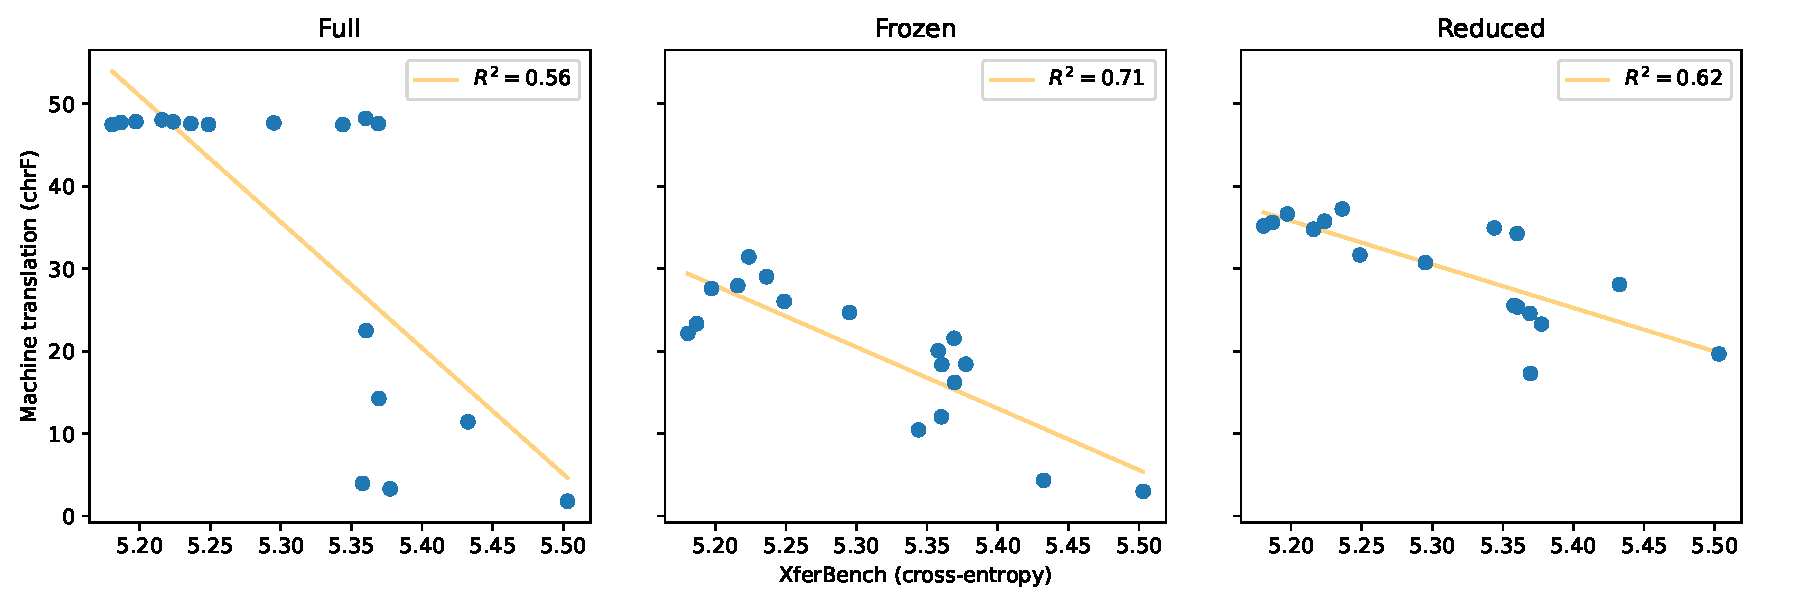
\includegraphics[width=\textwidth]{chapters/xferbench/src/figures/correlation}
  \caption{Scatter plots showing XferBench score versus machine translation score.}
  \unskip\label{fig:scatter}
\end{figure*}

\section{Cross-entropy confidence interval computation}
\unskip\label{sec:bootstrapping}

Let $s \in S$ and $t \in T$ represent source and target languages, respectively.
$h_{s,t}$ represents the test cross-entropy of a model pretrained on $s$ and evaluated on $t$.
As sated in \Cref{eq:hs}, the score on XferBench is the mean cross-entropy across all target languages:
\begin{align}
  h_{s} &= \mean_{t' \in T}\left( h_{s,t'}\right)
  .
\end{align}
We would like to calculate a confidence interval (i.e., $h^-_s$ and $h^+_s$) for a source language's mean cross-entropy using the different cross-entropies on the target languages (i.e., $h_{s,t}$ for $t \in T$), yet these samples are not i.i.d., since the mean of cross-entropy each \emph{target} language can vary.
Thus, if we would like to use bootstrapping to calculate confidence intervals, we must first normalize the cross-entropies.
Let $\hat h_{s,t}$ be the normalized score:
\begin{align}
  \hat h_{s,t} &= \frac{h_{s,t} - \mean_{s'\in S}\left(h_{s',t}\right)}{\stdev_{s'\in S}\left(h_{s',t}\right)}
  .
\end{align}
Given the normalized scores, we can now bootstrap in order to compute confidence intervals for $\hat h_s$ (i.e., in the normalized space).\footnote{This is not intended to be statistically rigorous. Our cross-entropies are unlikely to be normally distributed, but this still be helpful for generally gauging uncertainty.}
Let $\hat h^+_s$ and $\hat h^-_s$ be the upper and lower bounds of the confidence interval computed using bootstrapping in the normalized space.
We can now translate these back into the raw cross-entropy space using the means and standard deviations from before:
\begin{align}
  h^+_s &= \hat h^+_s \cdot \stdev_{s'\in S}\left(h_{s',t}\right) + \mean_{s'\in S}\left(h_{s',t}\right) \\
  h^-_s &= \hat h^-_s \cdot \stdev_{s'\in S}\left(h_{s',t}\right) + \mean_{s'\in S}\left(h_{s',t}\right)
  .
\end{align}

\section{Error analysis}
\unskip\label{sec:error-analysis}
In the \emph{Full} setting of the machine translation task, the \emph{Yao+} and \emph{Mu+, SW} settings perform worse than expected (\emph{a priori} and compared to the other results in the setting).
Validation loss converged while chrF and BLEU scores remained near zero.
We provide a couple examples (taken from the predefined test set of WMT 2014) of model output to provide some insight into the reason for this.
No post processing used, generation is capped at $50$ tokens, and ``\textbackslash{}u0000'' represent single non-printable characters.

\paragraph{Example 1}
\emph{Input}: ``And while Congress can't agree on whether to proceed, several states are not waiting.''

\emph{Reference}: ``Et tandis que les membres du Congrès n'arrivent pas à se mettre d'accord pour savoir s'il faut continuer, plusieurs États n'ont pas attendu.''

[Model pretrained on] \emph{French}:
``\#Et alors que le Congrès ne peut pas convenir de poursuivre, plusieurs États ne sont pas en attente. » (traduction libre) Le Parlement européen. Le Parlement européen est d’avis que le Parlement européen doit être en mesure de faire preuve\#''

\emph{Disc, large}:
``\#Et bien que le Congrès ne puisse pas convenir de la marche à suivre, plusieurs États ne sont pas en attente.\textbackslash{}u2028\textbackslash{}u2028[Traduit par la Rédaction]\textbackslash{}u2028(Traduit par la Rédaction)\textbackslash{}u2028(Tra\#''

\emph{Yao+}:
``\#Annexe II, par.\allowbreak{}\textbackslash{}xa02.\allowbreak{}2.\allowbreak{}2.\allowbreak{}2.\allowbreak{}2.\allowbreak{}2.\allowbreak{}2.\allowbreak{}2.\allowbreak{}2.\allowbreak{}2.\allowbreak{}2.\allowbreak{}2.\allowbreak{}2.\allowbreak{}2.\allowbreak{}2.\allowbreak{}2.\allowbreak{}2.\allowbreak{}2.\allowbreak{}2.\allowbreak{}2.\allowbreak{}2.\allowbreak{}\#''

\emph{Mu+, SW}:
``\#Annexe II.\allowbreak{}\textbackslash{}xa0\allowbreak{}\textbackslash{}xa0: Appendice I.\allowbreak{}\textbackslash{}xa0I.\allowbreak{}\textbackslash{}xa0I.\allowbreak{}\textbackslash{}xa0I.\allowbreak{}\textbackslash{}xa0I.\allowbreak{}\textbackslash{}xa0I.\allowbreak{}\textbackslash{}xa0I.\allowbreak{}\textbackslash{}xa0I.\allowbreak{}\textbackslash{}xa0I.\allowbreak{}\textbackslash{}xa0I.\allowbreak{}\textbackslash{}xa0I.\allowbreak{}\textbackslash{}xa0I.\allowbreak{}\textbackslash{}xa0I.\allowbreak{}\textbackslash{}xa0I\#''

\paragraph{Example 2}
\emph{Input}:
``This really is a must for our nation.''

\emph{Reference}:
``Cela est vraiment indispensable pour notre nation.''

\emph{French}:
``\#C'est vraiment une nécessité pour notre nation. Nous devons y parvenir. Nous devons y parvenir. Nous devons y parvenir. Nous devons y parvenir. Nous devons y parvenir. Nous devons y parvenir. Nous devons y parvenir. Nous devons y\#''

\emph{Disc, large}:
``\#C'est vraiment un devoir pour notre nation. C'est un devoir.\textbackslash{}u2028\allowbreak{}\textbackslash{}u2028(...)\allowbreak{}\textbackslash{}u2028\allowbreak{}\textbackslash{}u2028(...)\allowbreak{}\textbackslash{}u2028(...)\allowbreak{}\textbackslash{}u2028(...)\allowbreak{}\textbackslash{}u2028(...)\allowbreak{}\textbackslash{}u2028(...)\allowbreak{}\textbackslash{}u2028(...)\allowbreak{}\textbackslash{}u2028(\#''

\emph{Yao+}:
``\#Annexe II, par.\allowbreak{}\textbackslash{}xa02.\allowbreak{}2.\allowbreak{}2.\allowbreak{}2.\allowbreak{}2.\allowbreak{}2.\allowbreak{}2.\allowbreak{}2.\allowbreak{}2.\allowbreak{}2.\allowbreak{}2.\allowbreak{}2.\allowbreak{}2.\allowbreak{}2.\allowbreak{}2.\allowbreak{}2.\allowbreak{}2.\allowbreak{}2.\allowbreak{}2.\allowbreak{}2.\allowbreak{}2.\allowbreak{}\#''

\emph{Mu+, SW}:
``\#Annexe II.\allowbreak{}\textbackslash{}xa0\allowbreak{}\textbackslash{}xa0: Appendice I.\allowbreak{}\textbackslash{}xa0I.\allowbreak{}\textbackslash{}xa0I.\allowbreak{}\textbackslash{}xa0I.\allowbreak{}\textbackslash{}xa0I.\allowbreak{}\textbackslash{}xa0I.\allowbreak{}\textbackslash{}xa0I.\allowbreak{}\textbackslash{}xa0I.\allowbreak{}\textbackslash{}xa0I.\allowbreak{}\textbackslash{}xa0I.\allowbreak{}\textbackslash{}xa0I.\allowbreak{}\textbackslash{}xa0I.\allowbreak{}\textbackslash{}xa0I.\allowbreak{}\textbackslash{}xa0I\#''

\paragraph{Discussion}
Although all of the models have trouble terminating properly, the \emph{French} and \emph{Disc, large} models (which have high chrF scores) clearly condition their generation on the text, whereas \emph{Yao+} and \emph{Mu+, SW} give the same output regardless of the input.
Although this is unexpected, we can see in the \emph{Full} setting in \Cref{fig:scatter} that there is sharp drop off between high-performing and low-performing languages.
We suspect that the higher learning rate during tuning caused this bimodal distribution of results and is at least in part responsible for the poor performance \emph{Yao+} and \emph{Mu+, SW} models on the MT experiment's \emph{Full} setting.



\typeout{INFO: \arabic{comment} comments.}


 \typeout{INFO: \arabic{comment} comments.}
\end{document}
